\documentclass[11pt]{article}

\input{preamble} % If needed, you can load additional packages or
% define your own macros in the preamble.tex file

\title{VesSkel: Vessel Skeletonization and Graph-Based Phenotype Analysis in
Retinal Fundus Images}
\author{Simon Wittmann}

\affil{
  % [Master's / Bachelor's] thesis in [your study degree]\\ % For theses
  % Direct supervisor: [your direct thesis supervisor]\\ % For theses,
  % delete if directly supervised by David
  % Supervising professor: Prof. Dr. David B. Blumenthal\\ % For theses
  Project report\\ % For project reports in the module Project
  Biomedical Network Science\\
  %Student paper\\ % For student papers in the module Network Medicine
  Module title: Project Biomedical Network Science\\
  Semester: SS 2026\\
  Matriculation number: 23760671\\
  Biomedical Network Science Lab, Department Artificial Intelligence in
Biomedical Engineering, Friedrich-Alexander-Universität Erlangen-Nürnberg}

\date{Submission date: 2026-07-25}

\begin{document}

\maketitle

\begin{abstract}
  Quantitative analysis of network-like structures in biomedical
  images provides valuable morphological descriptors for a wide range
  of biological and clinical applications, including vascular
  analysis, neuronal morphology and filamentous tissue
  characterization. The standard workflow -- skeletonizing binary
  vessel segmentations to derive graph-based features -- requires
  assembling heterogeneous tools differing in license, dimensionality
  support, and interface, introducing reproducibility risks. To
  address this, we present VesSkel, an open-source-licensed Python
  package that unifies skeletonization, artifact removal, and
  phenotype feature extraction in a single end-to-end pipeline.
  VesSkel provides a Numba-parallelized Lee94 thinning implementation
  that is 5--9$\times$ faster in 2D (0.084\,s/image,
  $3504\times2336$\,px) and 1.8--2.0$\times$ faster in 3D
  (16.77\,s/image, $\sim430\times512\times512$\,voxels) than existing
  alternatives while producing bit-identical output, a novel
  junction-cleanup step that removes thinning-induced triangle
  artifacts, and dual napari and CLI interfaces with fully
  serializable JSON configuration for reproducible batch processing.
  From each image, VesSkel extracts 29 per-image features spanning
  topology, morphology, and density. On the High-Resolution Fundus
  dataset, an SVM trained on ANOVA-selected VesSkel features achieves
  91.1\% accuracy in discriminating healthy, diabetic retinopathy,
  and glaucoma subjects, confirming that its features encode
  biologically relevant vascular phenotypes.
\end{abstract}

\clearpage

\tableofcontents

\clearpage

\section{Introduction}\label{sec:introduction}

Quantitative analysis of vascular morphology from biomedical images
provides clinically relevant biomarkers for a wide range of
diseases~\cite{skel_survey}. Regardless of the imaging
modality or anatomical site -- whether in retinal fundus photography,
CT angiography of the lungs, or microscopy of tissue sections -- a
common approach~\cite{skel_survey} is to skeletonize the binary
vessel segmentation and then derive graph-based features from the
resulting one-pixel-wide centerline representation.

Several software tools have been developed for this task, including
REAVER~\cite{REAVER}, VesselVio~\cite{VesselVio},
VesselExpress~\cite{VesselExpress}, TWOMBLI~\cite{TWOMBLI},
VesSAP~\cite{VesSAP}, and Skan~\cite{Skan<3}. These tools differ
substantially as can be seen in Table~\ref{tab:tools-general}.

Despite their individual strengths, no existing tool
simultaneously offers (i)~a permissive (MIT) license, (ii)~support
for both 2D and 3D binary masks, (iii)~an interactive graphical
interface alongside a batch-processing CLI, and (iv)~a comprehensive
feature set that includes fractal dimension, per-segment radius
statistics, and automatic cleanup of skeletonization artifacts. This
fragmentation forces researchers to maintain heterogeneous,
multi-tool pipelines that hinder reproducibility and increase the
barrier to entry for quantitative vessel analysis.

\begin{table}[htb]
  \centering
  \caption{Comparison of Different Vessel Processing
  Tools}\label{tab:tools-general}
  \small
  \begin{tabularx}{\textwidth}{lXXXXXX}
    \toprule
    Feature & REAVER & VesselVio & VesselExpress & TWOMBLI & VesSAP & Skan\\
    \midrule
    2D/3D & 2D & both & 3D & 2D & 3D & both\\
    \midrule
    GUI/Interface & interactive Matlab GUI & PyQt5 standalone app +
    cli & Web App (Docker) and Napari Plugin & FIJI/ImageJ Plugin
    with guided param setup & CLI only & Napari Plugin and Python Package\\
    \midrule
    Input Type & Raw 2D fluorescent images & Pre-binarized datasets &
    Raw 3D Volumes & Raw 2D Images & Raw 3D Volume & Pre-skeletonized binary\\
    \midrule
    License & BSD 3.0 & GPLv. 3 & GPLv. 3 & ? & MIT & BSD 3-clause\\
    \midrule
    Segmentation & Auto (background sub + adaptive threshold +
    morphological) & None & Auto (dual Frangi filter + statistical
    threshold) & Auto (Steger ridge detection) & Auto (5-layer 3D
    CNN, transfer learning) & None (skeleton analysis only)\\
    \midrule
    Skeletonization & Matlab bwmorph & Lee94 (custom numba impl) &
    skimage lee94 & None & skimage lee94 & None\\
    \bottomrule
  \end{tabularx}
\end{table}

We present VesSkel, an MIT-licensed Python package for vessel
skeletonization and graph-based phenotype analysis. VesSkel
implements the Lee94 thinning algorithm~\cite{lee94} with Numba-based
parallelization, supporting both 2D and 3D binary masks. The output
is verified to be pixel-identical to scikit-image's Lee94
implementation. In both 2D and 3D benchmarks
(Section~\ref{sec:results:performance}), VesSkel is consistently
faster than scikit-image and VesselVio while producing correct
skeletons. Beyond thinning, VesSkel provides an end-to-end pipeline:
optional preprocessing (morphological closing and hole-filling),
Lee94 skeletonization, a novel junction-cleanup step that removes
thinning-induced triangle artifacts on the skeleton graph, graph
construction using Skan~\cite{Skan<3}, and extraction of per-image,
per-branch, and per-node features. The pipeline is accessible through
two complementary interfaces: a napari plugin for interactive
parameter tuning and a command-line interface for reproducible batch
processing with JSON-configurable settings.

We demonstrate VesSkel on the High-Resolution Fundus (HRF)
dataset~\cite{HRF}, which comprises 45 fundus images with manual
vessel segmentations from three clinical groups: 15 healthy subjects,
15 patients with diabetic retinopathy, and 15 patients with glaucoma.
From each image, we extracted vessel phenotype features and evaluated
their discriminative power achieving accurate discrimination between
the three groups (Section~\ref{sec:results:phenodiff}). These results
confirm that VesSkel captures biologically relevant differences in
vascular morphology.

In summary, our main contributions are: (1)~a Numba-parallelized
Lee94 thinning implementation for 2D and 3D data, validated for
correctness against scikit-image and benchmarked against existing
implementations; (2)~an integrated feature extraction pipeline with a
novel junction artifact cleanup mechanism; (3)~a dual-interface
design (napari plugin + CLI) with JSON-configurable reproducibility;
and (4)~a demonstration of phenotype differentiation and
classification on the HRF dataset. The remainder of this paper is
organized as follows. Section~\ref{sec:results} presents the pipeline
overview, skeletonization performance, feature summary, and phenotype
analysis results. Section~\ref{sec:discussion} discusses limitations
and future directions. Section~\ref{sec:methods} details the Lee94
algorithm, our implementation and test strategy, the cleanup
procedure, graph construction, and experimental setup.

\section{Results}\label{sec:results}

% \subsection{Structure of the Results section}\label{sec:results:overview}
%
% The first subsection of the \nameref{sec:results} is often used to
% provide a high-level overview of the entire work. This is typically
% supported by a visual overview in \Cref{fig:overview-placeholder}.
% The overview should enable readers to understand the material
% presented in the subsequent subsections of the \nameref{sec:results}
% section. The methodological details are then explained in a dedicated
% \nameref{sec:methods} section.
%
% \begin{figure}[htb]
%   \centering
%   \includegraphics[width=0.5\linewidth]{example-image-a}
%   \caption{Placeholder for a figure that visualizes the entire study.}
%   \label{fig:overview-placeholder}
% \end{figure}
%
% The remainder of the \nameref{sec:results} is typically structured
% into topical subsections. As a rule of thumb, each subsection should
% present one key finding, supported by one data figure. Of course, you
% can divert from this rule of thumb if it does not fit for your work.
%
% \subsection{Figures}\label{sec:results:figures}
%
% An example of a well-made data figure is shown in
% \Cref{fig:data-figure}. Please ensure that font sizes are large
% enough, that all colors are resolved with legends, and that all $x$-
% and $y$-axes are labeled. If possible, use vector graphics to avoid
% problems due to low resolutions. Add labels to the individual panels
% shown in your figure, which you can then use in your textual
% descriptions. E.\,g.: ``For the multi-class datasets LT1 and LT2
% (\Cref{fig:data-figure}B, C), differences in performance between the
% MLP and SOM classifiers are much more pronounced than for the binary
% datasets LT1b and LT2b (\Cref{fig:data-figure}E, F)''. Place the
% figures in the vicinity of the corresponding text by choosing the
% appropriate placement option. For instance, the placement option
% \verb|htb| used for \Cref{fig:data-figure} tells \LaTeX{} that the
% figure should be placed ``here'' (\verb|h|, preferred choice), at the
% top (\verb|t|, second choice), or at the bottom (\verb|b|, third choice).
%
% \begin{figure}[htb]
%   \centering
%   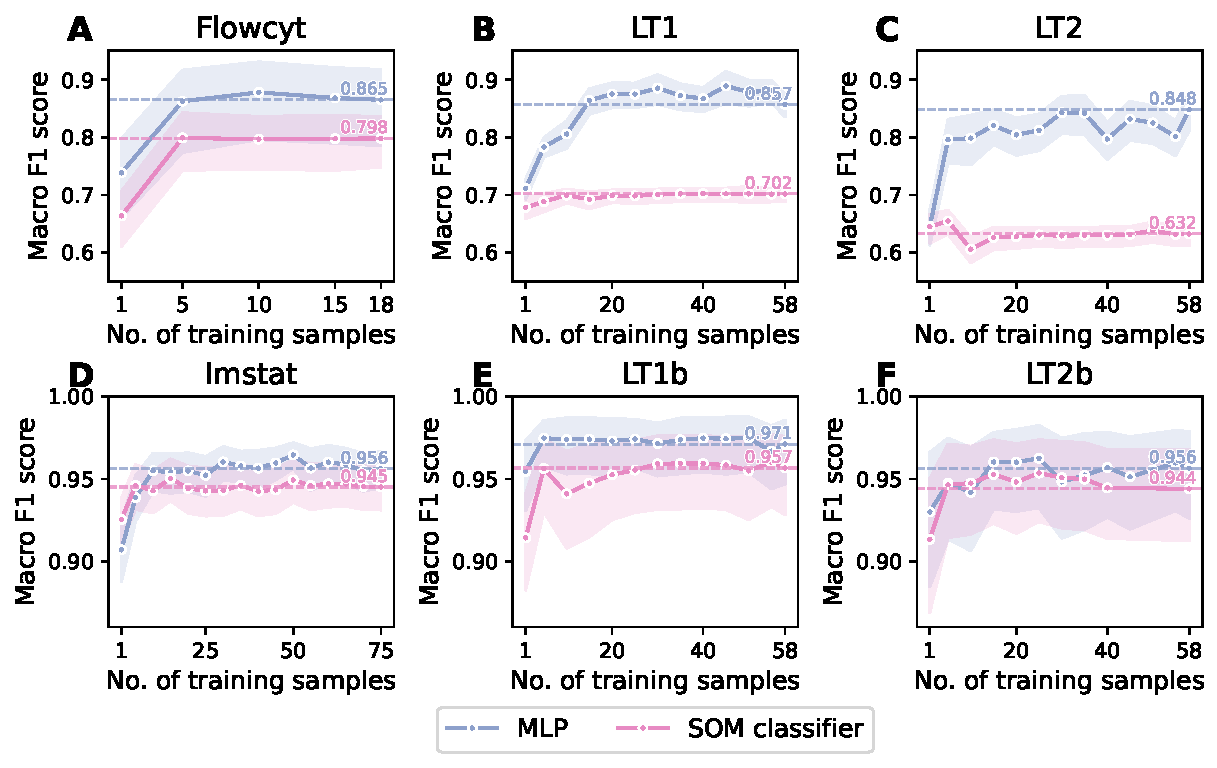
\includegraphics[width=\linewidth]{figures/example_figure.pdf}
%   \caption{Example of a data figure. Figure captions are placed below
%   the figures.}
%   \label{fig:data-figure}
% \end{figure}
%
% \subsection{References}\label{sec:results:references}
%
% References should be included using \verb|\textcite{ID}| and
% \verb|\cite{ID}| as in the following examples, (\verb|ID| is the
% handle of a publication defined in the file ``references.bib''). This
% produces references as in the following examples:
% \textcite{mcinnes2020umap} presented UMAP, a widely used
% dimensionality reduction method. scGPT \cite{Cui2024-km} is one of
% the earliest foundation models for single-cell RNA sequencing data.
%
% \subsection{Tables}\label{sec:results:tables}
%
% \begin{table}[htb]
%   \centering
%   \caption{Caption of \Cref{tab:supp-table}. Table captions are
%   placed above the tables.}
%   \label{tab:supp-table}
%   \begin{tabularx}{\linewidth}{lllX}
%     \toprule
%     Dataset & \# Samples & \# Features & Target variables \\
%     \midrule
%     D1 & 9473 & 187 & Five-year survival rate (binary) and overall
%     survival times (numeric)\\
%     D2 & 94734 & 1837 & Five-year survival rate (binary) and overall
%     survival times (numeric)\\
%     \bottomrule
%   \end{tabularx}
% \end{table}
%
% Nicely formatting tables with \LaTeX{} is a bit tricky, but it is
% possible. \Cref{tab:supp-table} shows an example that uses an
% \verb|X| column from the \verb|tabularx| environment for cells with
% automatic line break that adapt to the available horizontal space, as
% well as the \verb|\toprule|, \verb|\midrule|, and \verb|\bottomrule|
% commands from the \verb|booktabs| package. As for figures, use
% appropriate placement options to ensure that tables appear close to
% the corresponding text.

\subsection{Overview of the VesSkel Pipeline}\label{sec:results:overview}

\begin{figure}[htb]
  \centering
  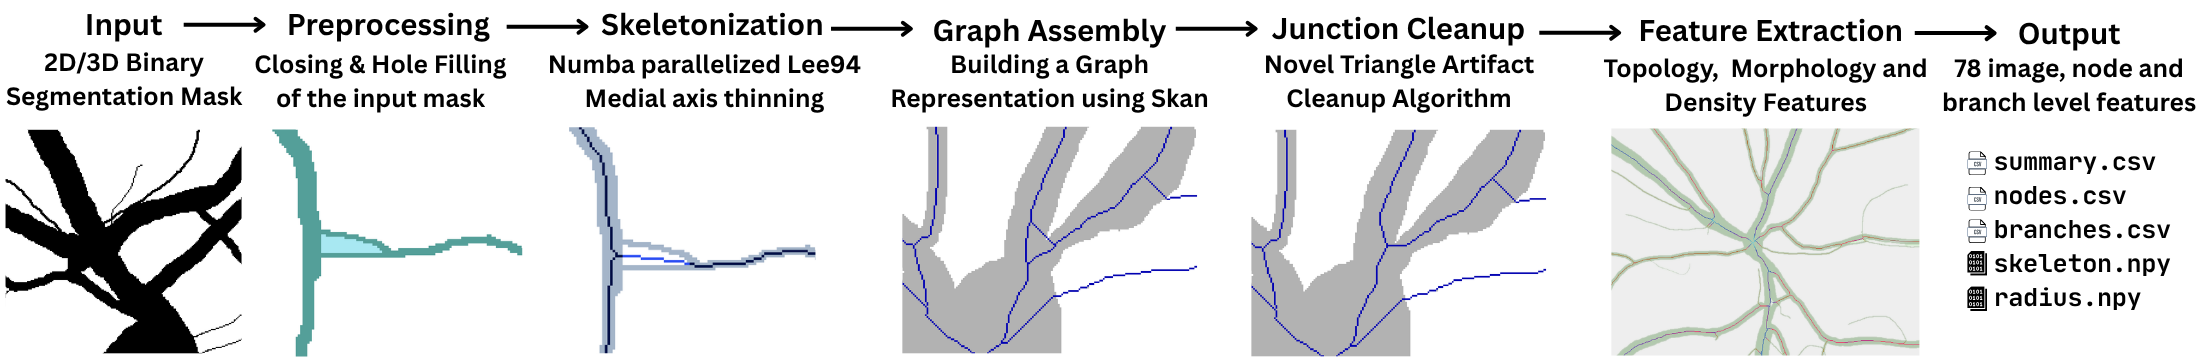
\includegraphics[width=1.0\linewidth]{figures/VesSkel_Pipeline_Advanced.png}
  \caption{Overview of the VesSkel end-to-end processing pipeline.
    Starting from a 2D/3D binary segmentation mask, the input undergoes
    optional preprocessing (morphological closing and hole filling)
    before skeletonization via the Lee94 thinning algorithm. After
    graph assembly using Skan and an optional junction cleanup to
    remove triangle artifacts, topological, morphological, and density
    features are extracted at three granularity levels (image, node,
  and branch) and exported as structured files.}
  \label{fig:pipeline}
\end{figure}

VesSkel provides an end-to-end pipeline from binary vessel masks to
quantitative phenotype features, as illustrated in
Figure~\ref{fig:pipeline}. The pipeline accepts pre-binarized vessel
segmentations and optionally applies preprocessing (morphological
closing and hole filling) to remove segmentation artifacts. The
cleaned mask is then skeletonized using the Lee94 thinning
algorithm~\cite{lee94}. An optional junction-cleanup step detects and
removes thinning-induced triangle artifacts from the skeleton graph.
The cleaned skeleton is converted to a graph representation using
Skan~\cite{Skan<3}, from which features are extracted at three
granularity levels: per-image summary statistics, per-branch
measurements, and per-node topological properties.

The pipeline is accessible through two complementary interfaces: a
napari plugin for interactive parameter tuning with real-time visual
feedback, and a command-line interface for reproducible batch
processing. All extraction parameters are serializable to a
configuration file, enabling full experiment reproducibility.

\subsection{Preprocessing and Artifact Removal}\label{sec:results:cleanup}

Binary vessel segmentations from automatic or manual annotation
frequently contain small holes and gaps, particularly in regions where
vessels are faint or at vessel crossings. During skeletonization, these
holes cause the thinning algorithm to trace circular paths around their
boundaries, producing spurious loops in the resulting skeleton graph.
To prevent such artifacts, VesSkel applies morphological closing
followed by hole filling as an optional preprocessing step before
thinning. The hole filling operation fills all enclosed background
regions in the mask. Holes exceeding a configurable size threshold are
reverted to preserve legitimate anatomical voids.

\begin{figure}[htb]
  \centering
  \begin{subfigure}[b]{0.3\linewidth}
    
\includegraphics[width=\linewidth]{../assets/hole_filling_input_mask.png}
    \caption{Input mask with hole}
    \label{fig:hole_filling:a}
  \end{subfigure}
  \hfill
  \begin{subfigure}[b]{0.3\linewidth}
    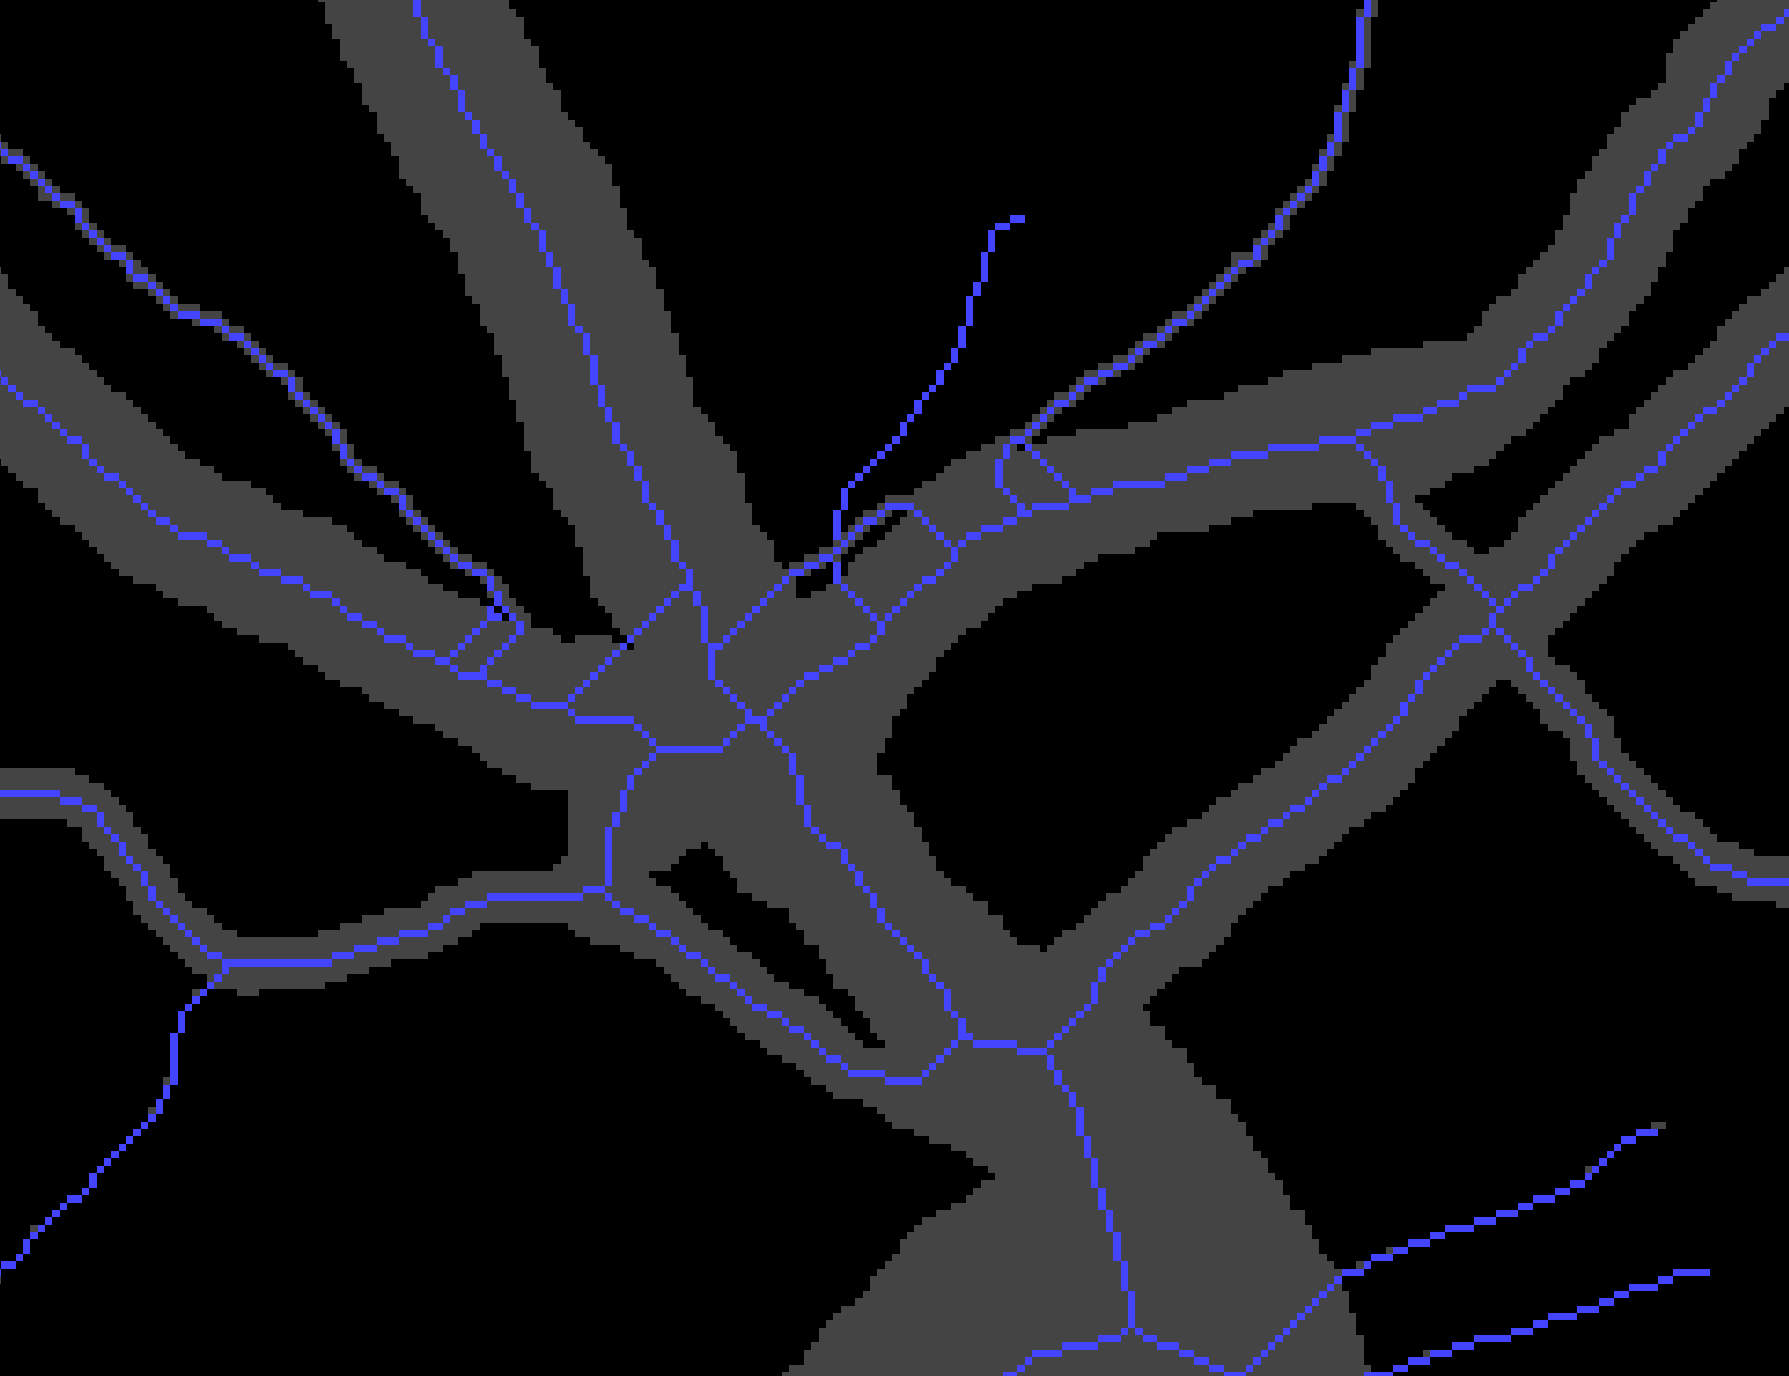
\includegraphics[width=\linewidth]{../assets/no_hole_filling_skeleton.png}
    \caption{Without hole filling}
    \label{fig:hole_filling:b}
  \end{subfigure}
  \hfill
  \begin{subfigure}[b]{0.3\linewidth}
    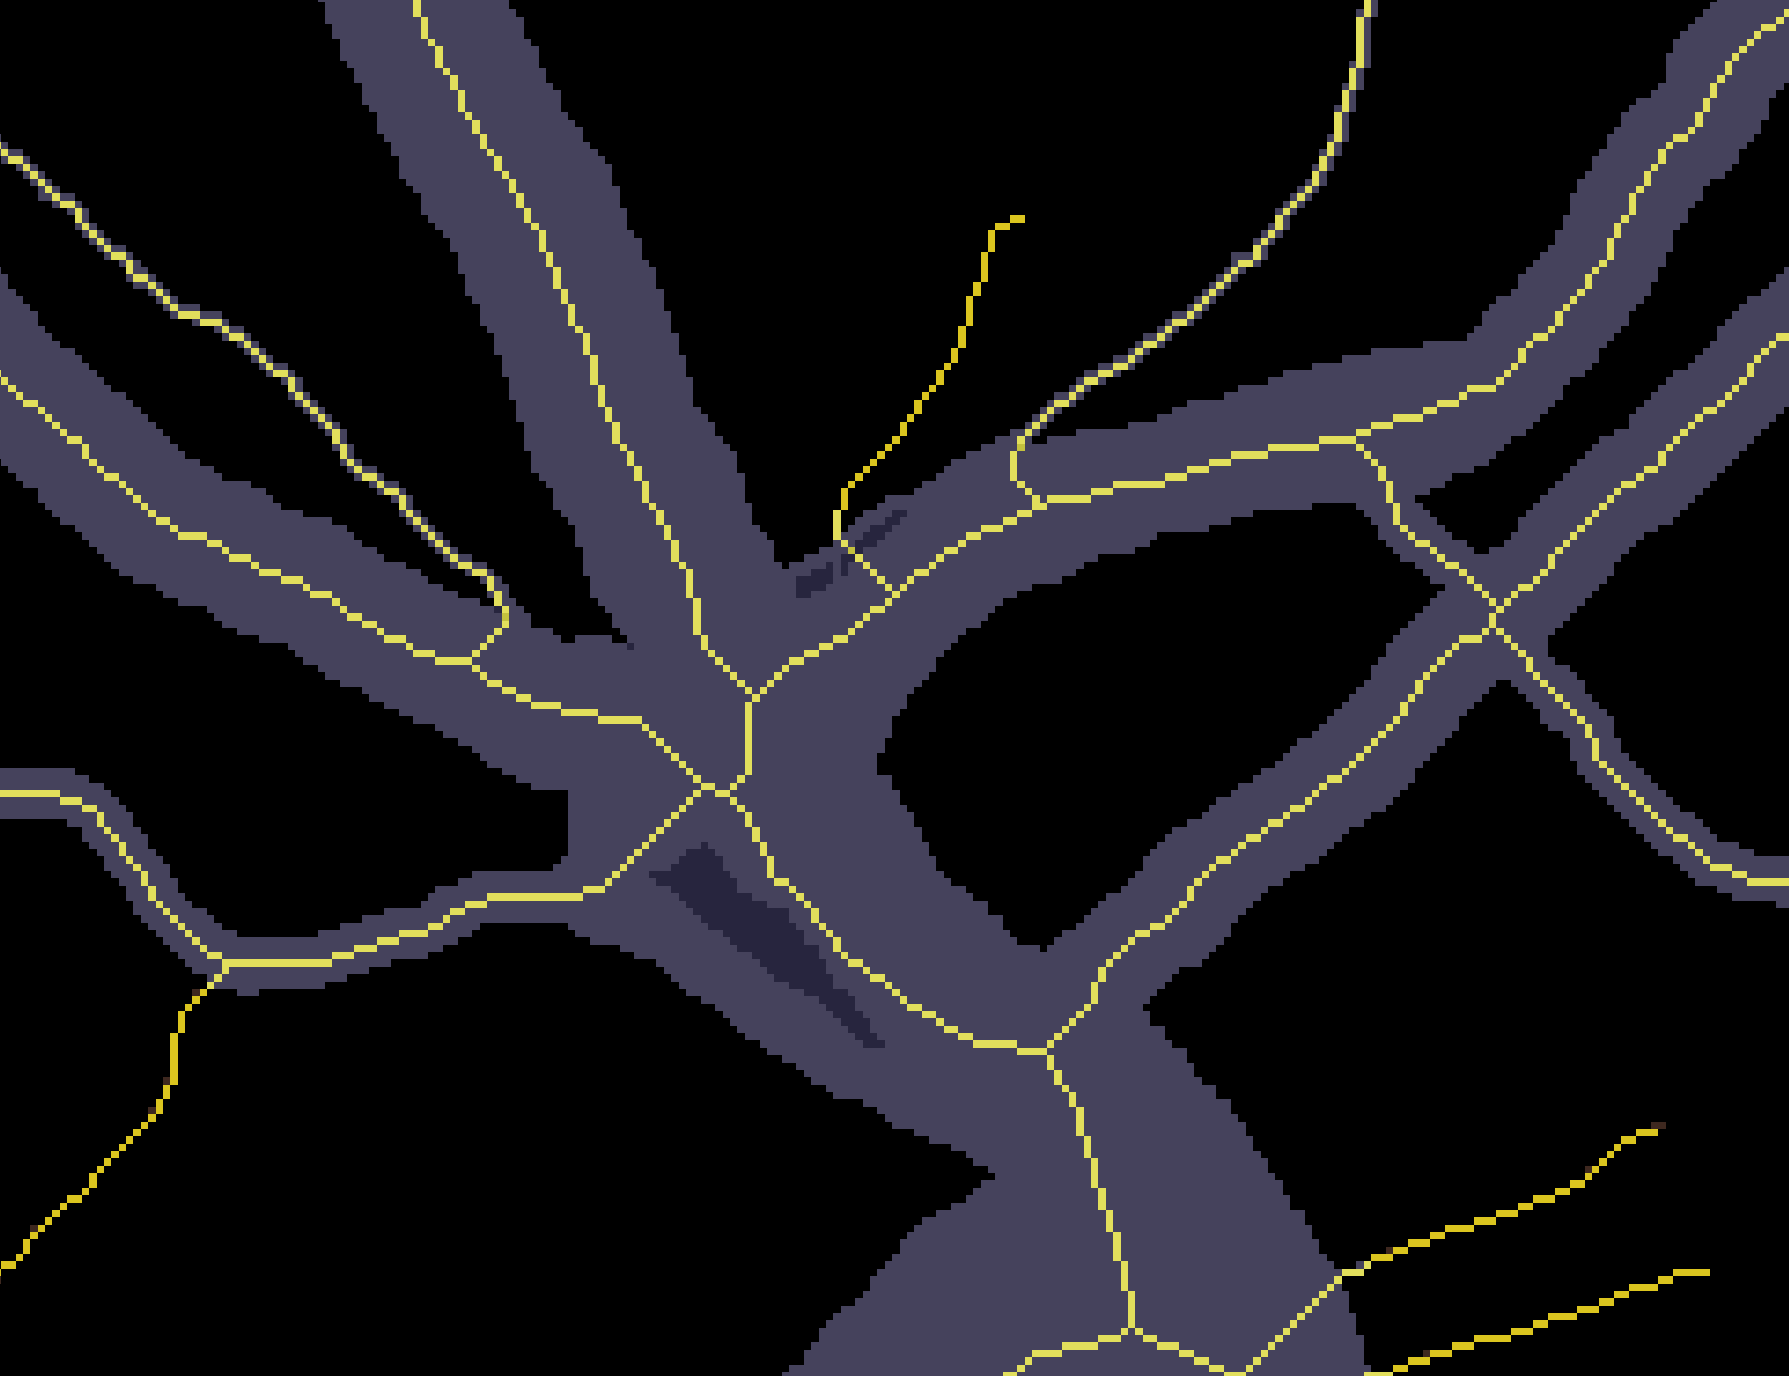
\includegraphics[width=\linewidth]{../assets/hole_filling_skeleton.png}
    \caption{With hole filling}
    \label{fig:hole_filling:c}
  \end{subfigure}
  \caption[Effect of hole filling on skeletonization quality]{Effect of
    hole filling on skeletonization quality. (a) Input segmentation mask
    with holes inside a vessel. (b) Without hole filling, the thinning
    algorithm traces the hole boundaries, creating circular skeleton
    artifacts. (c) After hole filling, the skeleton follows the correct
  vessel centerline.}
  \label{fig:hole_filling}
\end{figure}

Figure~\ref{fig:hole_filling} demonstrates the effect on a
representative region of an HRF fundus image. The input segmentation
mask (Figure~\ref{fig:hole_filling}a) contains holes in the vessel
segment, creating circular skeleton artifacts when thinned
directly (Figure~\ref{fig:hole_filling}b). With hole filling, the
skeleton follows the correct vessel centerline without spurious loops
(Figure~\ref{fig:hole_filling}c).

Despite preprocessing, a small number of artifacts may persist after
thinning. The most common are triangle/diamond artifacts at junction
points, which arise from the discrete marching behavior of the
thinning algorithm at bifurcation sites. VesSkel's optional junction
cleanup step detects these via the cycle basis of the skeleton graph.
For each cycle, the perimeter is compared to the local vessel diameter
estimated from the Euclidean distance transform at the cycle nodes.
Cycles whose perimeter is small relative to the local vessel diameter
are collapsed to a single pixel at their geometric centroid
(Figure~\ref{fig:junction_cleanup}b).

\begin{figure}[htb]
  \centering
  \begin{subfigure}[b]{0.3\linewidth}
    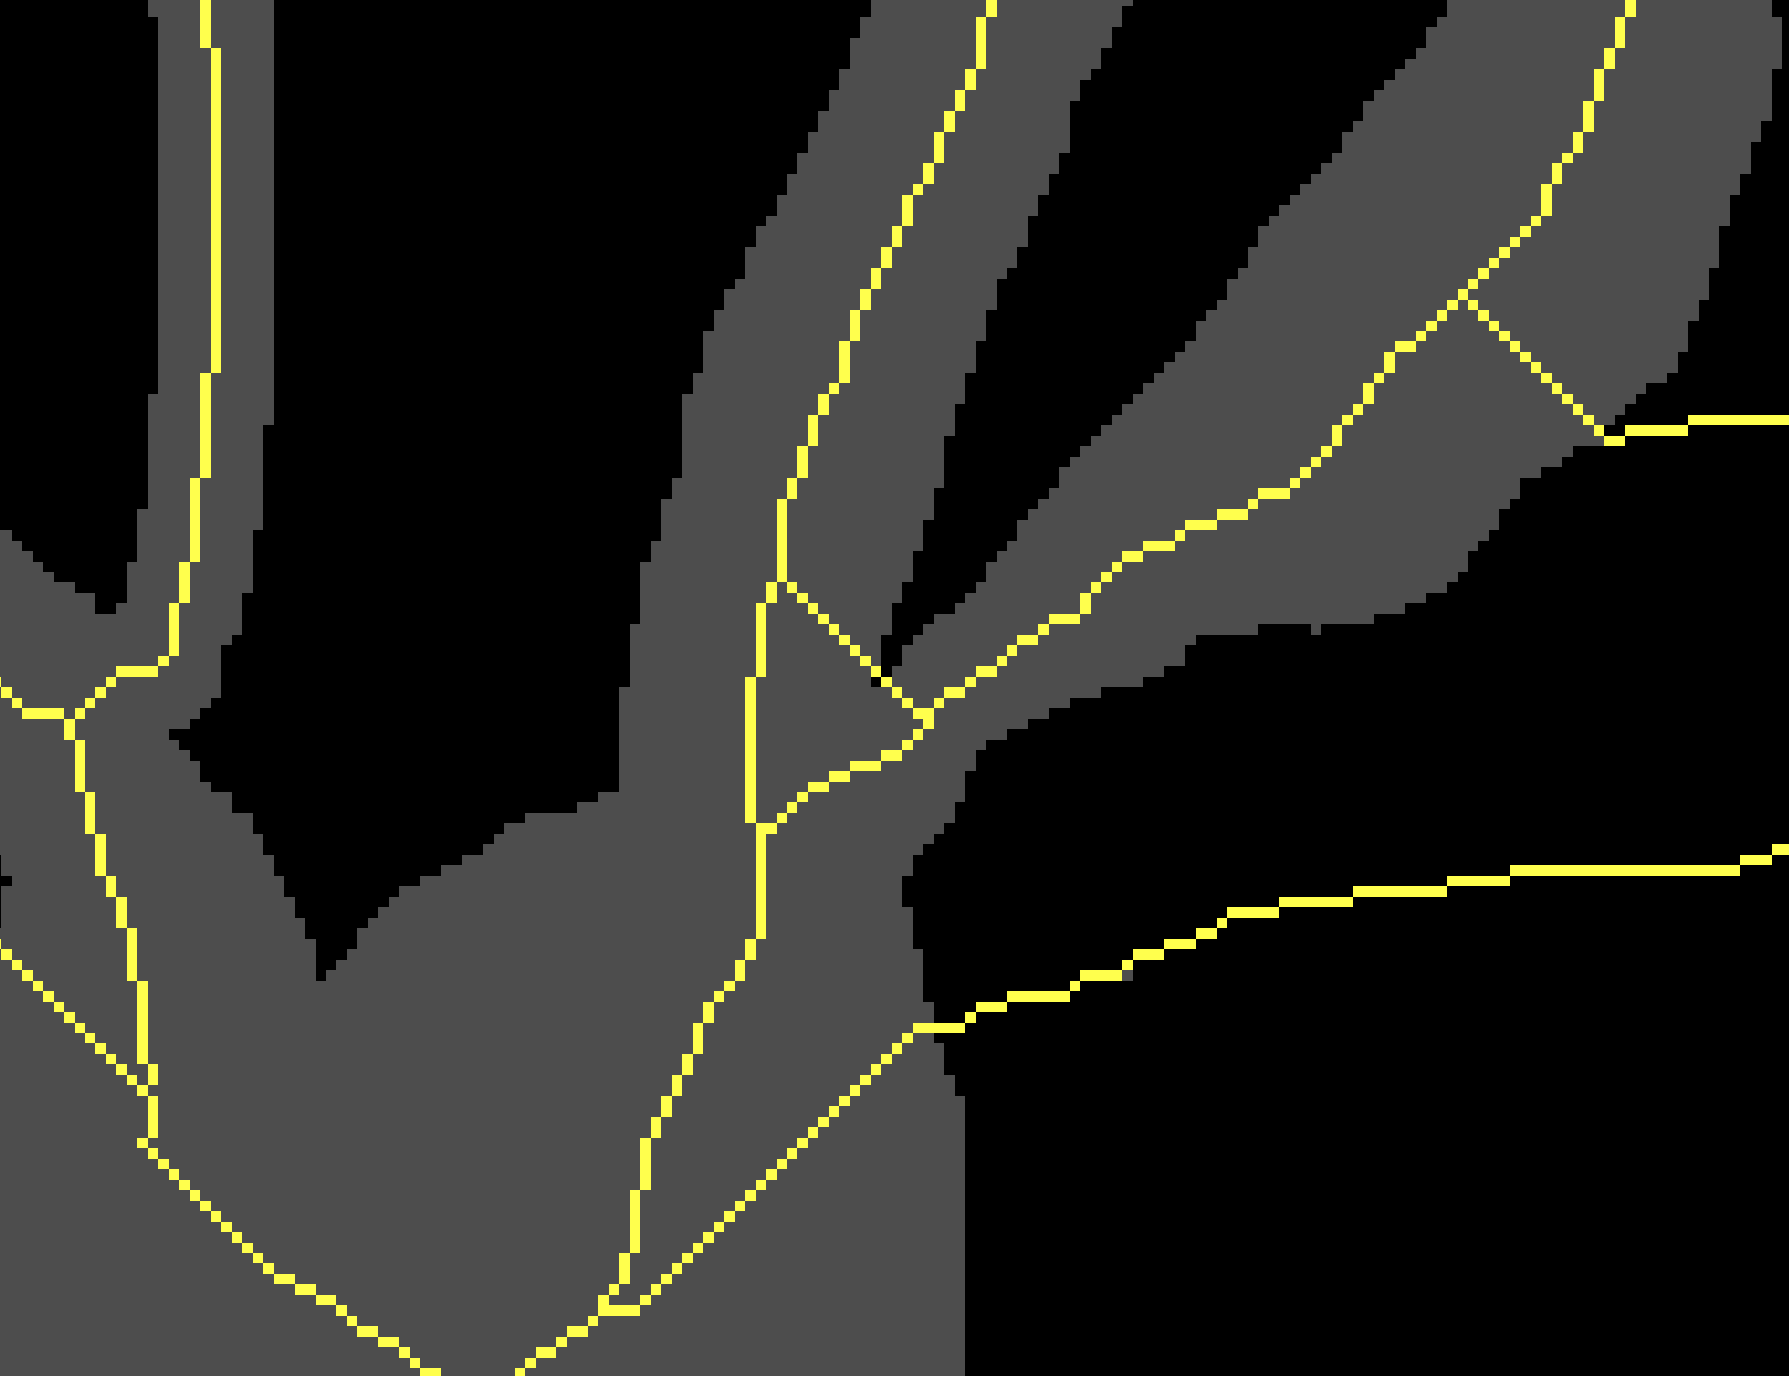
\includegraphics[width=\linewidth]{../assets/no_junction_cleanup.png}
    \caption{Before cleanup}
    \label{fig:junction_cleanup:a}
  \end{subfigure}
  \hspace{2em}
  \begin{subfigure}[b]{0.3\linewidth}
    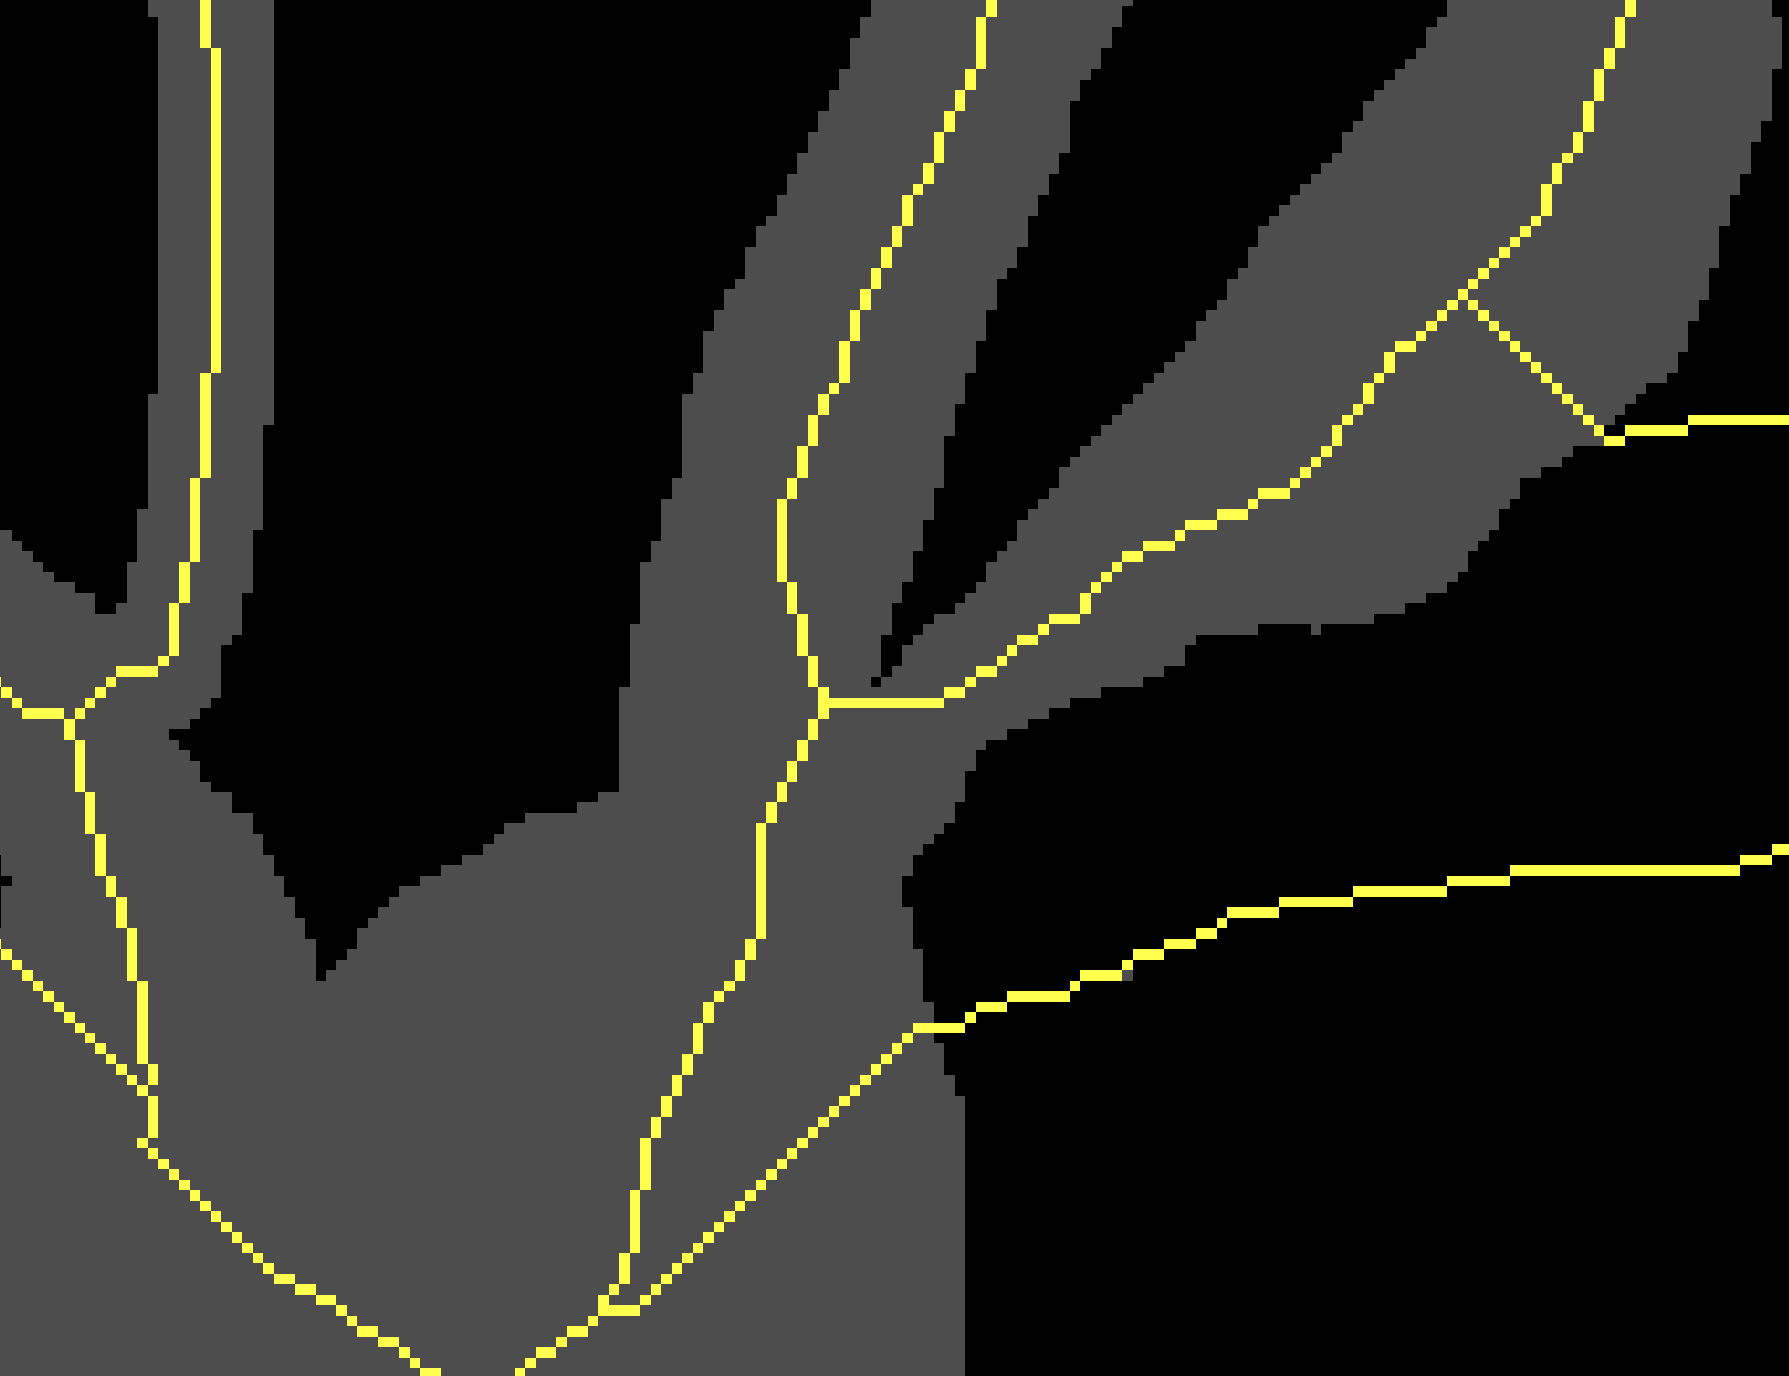
\includegraphics[width=\linewidth]{../assets/junction_cleanup.png}
    \caption{After cleanup}
    \label{fig:junction_cleanup:b}
  \end{subfigure}
  \caption[Junction cleanup removes triangle artifacts]{Junction
    cleanup removes triangle artifacts. (a) A triangle artifact at
    a vessel bifurcation after thinning. (b) After cleanup, the artifact
    is removed and the skeleton correctly represents the bifurcation
  topology.}
  \label{fig:junction_cleanup}
\end{figure}

A key observation from our experiments is that hole filling alone
resolves the vast majority of skeletonization artifacts before they
appear in the graph. When preprocessing is active, junction cleanup
becomes redundant for most images. This makes mask-level
preprocessing the primary and most effective defense against thinning
artifacts, with junction cleanup serving as a secondary safety net
for the remaining edge cases.

\subsection{Skeletonization Performance}\label{sec:results:performance}

We evaluated VesSkel's thinning performance on 2D and 3D data against
three competing implementations: scikit-image's~\cite{skimage}
Lee~\cite{lee94} and Zhang~\cite{zhang84} methods, and VesselVio's
Lee94 implementation~\cite{VesselVio}.

For 2D evaluation we used the full HRF dataset (45 images, $3504
\times 2336$~px each). Table~\ref{tab:perf-2d} reports the mean
thinning time per image. VesSkel achieves a mean of 0.084~s,
outperforming the next-fastest implementation (scikit-image Zhang,
0.157~s) by 1.87$\times$. Compared to the widely used Lee94 baseline
in scikit-image (0.438~s), VesSkel is 5.21$\times$ faster; against
VesselVio's Lee94 (0.796~s) the speedup reaches 9.46$\times$.

\begin{table}[htb]
  \centering
  \caption{2D thinning benchmark on the HRF dataset (45 images).}
  \label{tab:perf-2d}
  \small
  \begin{tabularx}{0.5\linewidth}{lcc}
    \toprule
    Implementation & Mean time (s) & vs.\ VesSkel \\
    \midrule
    VesSkel (Lee94)     & 0.084 & ---   \\
    skimage Zhang       & 0.157 & 1.87$\times$ slower \\
    skimage Lee         & 0.438 & 5.21$\times$ slower \\
    VesselVio Lee94     & 0.796 & 9.46$\times$ slower \\
    \bottomrule
  \end{tabularx}
\end{table}

For 3D evaluation we used 20 lung CT masks from the VESSEL12
challenge (~$430\times512\times512$~voxels, $\sim$12\% mean
foreground fraction). Per-scan thinning times are shown in
Table~\ref{tab:perf-3d}.~VesSkel achieves a mean of 16.77~s,
outperforming scikit-image Lee (30.25~s, 1.80$\times$) and
VesselVio~Lee94 (33.97~s, 2.03$\times$).

\begin{table}[htb]
  \centering
  \caption{3D thinning benchmark on the VESSEL12 lung CT dataset
  (20 scans).}
  \label{tab:perf-3d}
  \small
  \begin{tabularx}{0.5\linewidth}{lcc}
    \toprule
    Implementation & Mean time (s) & vs.\ VesSkel \\
    \midrule
    VesSkel (Lee94)   & 16.77 & ---   \\
    skimage Lee       & 30.25 & 1.80$\times$ slower \\
    VesselVio Lee94   & 33.97 & 2.03$\times$ slower \\
    \bottomrule
  \end{tabularx}
\end{table}

Critically, VesSkel sacrifices no correctness for speed. The output
is~\textbf{bit-identical} to scikit-image's Lee94 implementation.
This was verified via the regression test suite described in
Section~\ref{sec:methods:impl:tests}.

Beyond per-image thinning, the \texttt{vesskel run} CLI supports
parallel batch processing. On a 12-core homogeneous workstation,
processing all 20 VESSEL12 scans took 4:53.63~min with a single
worker and 3:28.94~min with 12 workers (1.41$\times$ speedup, 1153\%
CPU utilization). The sub-linear speedup occurs because we already
parallelize the thinning of each individual image using Numba.

\subsection{Skeleton and Graph Features}\label{sec:results:features}

Table~\ref{tab:feature-comparison} surveys 78 individual feature rows
across seven vasculature analysis tools. VesSkel extracts 29 per-image
summary features spanning three core dimensions of vessel phenotype
analysis: topology, morphology, and density.

Topology features describe the graph structure of the vascular
network---node count, edge count, endpoint count, bifurcation count,
connected components, and degree statistics. Morphology features capture
the shape of individual vessel segments---length statistics (total,
mean, standard deviation, minimum, maximum), tortuosity (mean and
standard deviation), fractal dimension (box-counting estimate with
R$^2$ fit quality), hyphal growth unit, and radius and diameter
statistics (mean, standard deviation, minimum, maximum). Density
features quantify vascular coverage---total vessel area and vessel area
fraction within the field of view. Beyond these per-image summaries,
VesSkel also outputs per-branch measurements (radius, diameter, volume,
surface area, tortuosity for each segment) and per-node properties
(degree, endpoint/junction classification, local radius), enabling
localized analyses. The technical details of graph construction and
feature computation are given in
Section~\ref{sec:methods:graph}.

\subsection{Phenotype Differentiation}\label{sec:results:phenodiff}

We assessed whether the 29 per-image summary features capture
biologically relevant differences between the three clinical groups
using one-way ANOVA (details in \Cref{sec:methods:setup:phenodiff}).
The most discriminating features were mean radius and mean diameter
(both F=114.3, $p \approx 10^{-17}$), followed by mean segment volume
(F=43.7, $p \approx 10^{-11}$) and vessel area and vessel area
fraction (F=39.1, $p \approx 10^{-10}$, \Cref{fig:anova}).

\begin{figure}[htb]
  \centering
  
\includegraphics[width=0.85\linewidth]{figures/feature_difference_anova.pdf}
  \caption{Top ten features ranked by ANOVA F-statistic for
  differences among the three phenotypes.}
  \label{fig:anova}
\end{figure}

Examination of group means reveals a consistent phenotypic ordering:
healthy retinas exhibit the largest mean vessel radius ($5.39 \pm
0.41$~px) and highest vascular density (vessel area fraction $0.093
\pm 0.009$), glaucoma subjects show the thinnest vessels across all
metrics (mean radius $3.86 \pm 0.19$~px; vessel area fraction $0.069
\pm 0.006$), and diabetic retinopathy subjects occupy an intermediate
position with respect to the vessel radius. This gradient mirrors the
clinical expectation that both conditions induce vascular remodeling
through distinct pathological
mechanisms~\cite{popovic_regional_2019}. The full set of group-wise
means for the top ten features is reported in
\Cref{tab:top-anova-feature-means}.

Many features exhibit strong mutual correlations, reflecting inherent
redundancy among morphological measurements of the same vascular
network. The correlation structure supports dimensionality reduction
for the classification task in the following section.

\subsection{Phenotype Classification}\label{sec:results:phenoclass}

To evaluate the predictive power of the extracted feature set, we
trained and compared five classifiers using stratified 5-fold
cross-validation: support vector machine (SVM), logistic regression,
random forest, a voting ensemble, and a stacking ensemble (details in
\Cref{sec:methods:setup:phenoclass}). Features were reduced to the
top ten by ANOVA F-statistic and standardized within each training
fold to prevent data leakage.

SVM with a linear kernel achieved the highest mean accuracy of
91.1\%, outperforming logistic regression (88.9\%), the voting and
stacking ensembles (both 84.4\%), and random forest (82.2\%)
(\Cref{fig:model-comparison}).

\begin{figure}[htb]
\centering

\includegraphics[width=0.6\linewidth]{figures/final_model_comparison.pdf}
\caption{Classification performance (mean accuracy $\pm$~SD) across
five models with stratified 5-fold cross-validation on the HRF dataset.}
\label{fig:model-comparison}
\end{figure}

Confusion matrices for each classifier are shown in the appendix
(\Cref{fig:confusion-matrices}). An analysis of SVM accuracy across
different numbers of selected features (appendix
\Cref{fig:svm-k-sweep}) confirms that the top ten features provide the
highest test-accuracy.

These results demonstrate that the captured features encode relevant
phenotype information, and that a linear SVM operating on a compact
feature subset can reliably distinguish the three clinical groups.

\section{Discussion}\label{sec:discussion}

We presented VesSkel, a unified pipeline for skeletonization and
phenotype feature extraction from binary vessel masks. On the HRF
dataset, VesSkel features achieved 91.1\% accuracy in discriminating
healthy, diabetic retinopathy, and glaucoma subjects, confirming
biological relevance of the extracted features.

Mask-level preprocessing (hole filling) proved more effective than
graph-level junction cleanup for removing skeletonization artifacts.
Our proof of Euler invariant redundancy in 2D Lee94 thinning
simplified the implementation and contributed to the measured
speedups. On the VESSEL12 lung CT benchmark, VesSkel achieved
consistent 1.8--2.0$\times$ speedups over skimage and VesselVio,
demonstrating effective 3D performance on clinically representative
volumes. A wavefront-based parallel deletion scheme could further
reduce the sequential bottleneck in the 3D removal phase.

The main limitations are the small single-dataset evaluation (HRF, 45
images), the lack of 3D phenotype validation, and the cross-sectional
design that precludes assessment of longitudinal sensitivity. The
junction cleanup collapses detected triangles to a single centroid
pixel and reconnects all attached branches to that point, which can
distort topology when branches have different calibers. Reconnecting
to the branch with the highest radius instead of the centroid may
preserve vessel hierarchy better. Future work should address the
remaining limitations through multi-site validation, 3D extension,
improved artifact detection, and longitudinal data.

\section{Methods}\label{sec:methods}

% \subsection{Structure of the Methods section}
%
% Good Methods sections are designed in such a way that the subsection
% headings allow the reader to quickly navigate it without reading the
% entire section from top to bottom. You may think of it as a
% dictionary where readers look up details of the work that are of
% particular interest to them. Each individual subsection should be
% detailed enough to allow replication of your work, so be precise in
% your descriptions. Overall, the subsections of your Methods section
% should cover all methodological details that are relevant for your
% work: details on your ML model or algorithm, descriptions of datasets
% and data preprocessing, details on evaluation protocols and metrics,
% description of competitor approaches, etc.
%
% \subsection{Equations}
%
% When using mathematical formalism, make sure that you always define
% all symbols, including indices. For instance, if for some reason you
% want to introduce the quantity $s$ as the sum of all Fibonacci
% numbers $F_i$ with odd indices smaller or equal to $100$, you should
% not simply write
% \begin{equation}
%   s=\sum_{i}F_i \label{eq:bad}
% \end{equation}
% and hope that the range of the index $i$ is clear from the context.
% Instead, introduce an index set
% $\mathcal{O}_{100}=\{i\in\mathbb{N}\mid i\leq100\land\text{$i$ is
% odd}\}$ and define $s$ as in the following \Cref{eq:good}:
% \begin{equation}
%   s=\sum_{i\in\mathcal{O}_{100}}F_i \label{eq:good}
% \end{equation}
%
% Moreover, it is preferable to always use numbered instead of
% unnumbered equation environments (i.\,e.,
%   \verb|\begin{equation}...\end{equation}| and
%   \verb|\begin{align}...\end{align}| instead of
%   \verb|\begin{equation*}...\end{equation*}| and
% \verb|\begin{align*}...\end{align*}|). Like this, you can reference
% the equations in the text and it is easier for readers to refer to them.
%
% \subsection{Theorems, definitions, proofs, and similar environments}
%
% This template provides \verb|definition|, \verb|observation|,
% \verb|remark|, \verb|proposition|, \verb|lemma|, \verb|theorem|, and
% \verb|proof| environments you can use as needed. Examples are
% provided in \Cref{def:dummy-def} and \Cref{thm:dummy-theorem}.
%
% \begin{definition}[Optional name of defined concept]\label{def:dummy-def}
%   Statement of the definition.
% \end{definition}
%
% \begin{theorem}[Optional name of theorem]\label{thm:dummy-theorem}
%   Statement of the theorem.
% \end{theorem}
%
% \begin{proof}
%   Proof here.
% \end{proof}

\subsection{Lee94 Thinning Algorithm}\label{sec:methods:lee}

The Lee94 algorithm~\cite{lee94} produces topologically
preserving skeletons by iteratively removing border voxels from a
binary shape until only a one-voxel-wide medial axis remains. In each
sub-iteration, a border voxel is removed only if it satisfies up to
four criteria:
(1)~it is a \textbf{border point} (at least one 4-neighbor in 2D or
6-neighbor in 3D is background),
(2)~it is \textbf{not an endpoint} (more than one foreground neighbor
in the 8-neighborhood for 2D or 26-neighborhood for 3D),
(3)~removing it leaves the \textbf{Euler
characteristic}~\cite{lee_winding_1991} unchanged
($\Delta\chi = 0$, preventing hole or tunnel creation), and
(4)~it is a \textbf{simple point} (the foreground neighbors form a
single connected component, preventing disconnection).

In 3D, all four criteria are active and the algorithm proceeds through
six directional sub-iterations (north, south, east, west, up, down).
Criteria~(3) and~(4) are complementary in 3D: the Euler invariant
detects the creation or destruction of tunnels, while the simple-point
condition prevents disconnection of the foreground object.

In 2D, only four directions (north, south, east, west) are needed and
condition~(3) is provably redundant (Section~\ref{sec:methods:impl:deviations}).
The border-point and simple-point conditions together guarantee
$\Delta\chi = 0$, allowing the Euler check to be omitted entirely.

\subsection{Implementation Details}\label{sec:methods:impl}

\paragraph{Deviations of this Implementation}\label{sec:methods:impl:deviations}

Our 2D implementation differs from the canonical Lee94 algorithm in
two important ways. First, we proved that the Euler invariant check
is redundant in 2D (full proof in the project documentation). In 2D,
a hole cannot be created by removing a border point (any border point
has at least one background 4-neighbor, providing an escape path), and
a hole cannot be eliminated by removing a simple point (the
simple-point condition already prevents disconnection). Since
$\Delta\chi = \Delta O - \Delta H$ and $\Delta H = 0$ always holds,
the simple-point condition ($\Delta O = 0$) guarantees $\Delta\chi =
0$. Omitting the Euler check removes the need for octree construction
and Euler LUT lookups, contributing directly to the 2D speedups
reported in Section~\ref{sec:results:performance}.

Second, 2D images are processed natively as 2D arrays rather than
embedded in a 3D volume. This collapses the 26-neighborhood to an
8-neighborhood, reduces border detection from six directions to four,
and halves memory usage.

\paragraph{2D Implementation}\label{sec:methods:impl:2d}

Our 2D implementation replaces the flood-fill DFS used in the
canonical simple-point check with a look-up table. The simple-point
condition requires counting connected foreground components in the
8-neighborhood of the candidate pixel. Since there are only $2^8 =
256$ possible 8-neighborhood patterns, we precompute the simple-point
status for every pattern at module-load time and store it in a
256-entry boolean LUT. During thinning, each candidate's eight
neighbors are packed into an 8-bit index and the verdict is read in
O(1) time, replacing an O(k) DFS traversal per candidate. The LUT is
compiled once by Numba's JIT and cached across all thinning calls.

The thinning loop iterates over four directional passes (north,
south, east, west) in each epoch. Each pass uses a two-phase
strategy. In the first phase, candidate collection is parallelized
over image rows using Numba's \texttt{prange}: each row independently
tests every foreground pixel against the border, endpoint, and
simple-point criteria and writes qualifying candidates into a per-row
buffer. Per-row buffers are then merged into a flat candidate list.
In the second phase, candidates are processed sequentially---a
pixel's deletion affects the neighborhood of adjacent candidates,
creating an inherent data dependency. Each candidate is re-checked
against the simple-point LUT and deleted if still valid. The
algorithm terminates when an entire pass over all four directions
yields no removable pixels.

\paragraph{3D Implementation}\label{sec:methods:impl:3d}

The 3D implementation started as a faithful port of scikit-image's
Cython Lee94 to pure Python with Numba acceleration. All four Lee94
criteria are active. The Euler invariant is computed using a
precomputed 256-entry LUT~\cite{lee94}: for each of the eight octants
of the $3\times3\times3$ neighborhood, seven neighbor occupancies are
packed into a 7-bit index, and the $\Delta\chi$ contribution is read
from the LUT. The simple-point condition is evaluated by counting
connected components among the 26 exterior voxels using DFS on a
precomputed 26-adjacency graph that records which pairs of neighbor
positions are themselves 26-adjacent---avoiding redundant distance
computations at runtime. The 3D border-point and endpoint checks
follow the standard Lee94 definition.

Candidate finding is parallelized over z-slices using a two-pass
scheme: each slice independently counts border voxels in parallel, a
prefix-sum computes write offsets, and each slice fills its
contiguous segment of the candidate array. Candidate marking is then
parallelized across all candidates with \texttt{prange}, where each
thread loads the $3\times3\times3$ neighborhood and evaluates all
four criteria. The removal phase is sequential.

A further optimization reduces redundant simple-point re-checks
during the removal phase. Since \texttt{mark\_removable\_candidates}
already verified every candidate against the current volume state
before any removals, the verdict remains valid for any candidate
whose 26 neighbors have not been modified. An epoch
counter---monotonically increasing per batch---is stamped onto every
removed voxel. During sequential removal, each candidate scans its 26
neighbors for a stamp matching the current epoch; if none is found,
the precomputed verdict is reused and the DFS is skipped. This avoids
O(26) DFS traversals for unaffected candidates and contributes to
VesSkel being competitive with existing 3D implementations.

\paragraph{Correctness Verification}\label{sec:methods:impl:tests}

We verify that VesSkel produces correct skeletons at two levels. For
both 2D and 3D, the output is pixel-identical to
\\\texttt{skimage.morphology.skeletonize(method='lee')} on all 45 HRF
images (2D) and the scikit-image brain volume~\cite{skimage} (3D).
Both are enforced by automated tests. Beyond that, a regression test
suite with saved baselines (skeletons and downstream extracted
features) detects unintended changes. The full test suite comprises
11 files containing 210 test cases covering thinning correctness,
feature extraction, pipeline toggles, CLI behavior, napari layer
generation, and config validation.

\subsection{Cleanup Steps}\label{sec:methods:cleanup}

Binary vessel masks frequently contain small holes and gaps
introduced during segmentation that would produce circular skeleton
artifacts during thinning (Section~\ref{sec:results:cleanup}).
VesSkel addresses these through optional preprocessing operations
applied before skeletonization. Hole filling
(\texttt{scipy.ndimage.binary\_fill\_holes})~\cite{scipy} fills all enclosed
background regions in the mask. To preserve legitimate anatomical
voids, the \texttt{max\_hole\_size} parameter reverts filled holes
whose area exceeds a configurable threshold. VesSkel also offers
morphological closing (\texttt{scipy.ndimage.binary\_closing}) as an
additional preprocessing step; however, on the HRF dataset
experiments showed no noticeable improvement over hole filling alone,
so closing was disabled (\texttt{closing\_iterations = 0}) in our
experiments. We used \texttt{max\_hole\_size = 300}.

Some thinning-induced artifacts, particularly small triangle
structures at bifurcation points, may survive mask-level
preprocessing. VesSkel removes these by analyzing the skeleton graph
after thinning. The skeleton is converted to a NetworkX graph $G =
(V, E)$ via Skan's \texttt{skeleton\_to\_nx} function~\cite{Skan<3},
and all elementary cycles $\mathcal{C}$ are enumerated using
\texttt{networkx.\\cycle\_basis}~\cite{networkx}. For a cycle $c =
(v_1, \dots, v_n)
\in \mathcal{C}$ with $v_{n+1} = v_1$, the perimeter is
\[
P(c) = \sum_{i=1}^{n} \lVert \operatorname{pos}(v_{i+1}) -
\operatorname{pos}(v_i) \rVert_2
\]
and the local vessel diameter is estimated as
\[
D(c) = \frac{2}{n} \sum_{i=1}^{n}
\operatorname{EDT}(\operatorname{pos}(v_i)),
\]
where $\operatorname{pos}(v)$ gives the pixel coordinates of node $v$
and $\operatorname{EDT}$ is the Euclidean distance transform of the
vessel mask. A cycle is classified as an artifact if
\[
P(c) < \tau \cdot D(c)
\]
with a default threshold of $\tau = 2.5$. Each such cycle --- or
connected group of overlapping cycles --- is collapsed to a single
pixel at its geometric centroid. External edges previously connected
to the removed nodes are reconnected to this centroid via Bresenham
line rasterization, preserving graph connectivity.

\subsection{Graph Construction and Features}\label{sec:methods:graph}

VesSkel converts the cleaned binary skeleton into a graph
representation using Skan's \texttt{Skeleton} object
\cite{Skan<3}, which builds a sparse adjacency matrix where each
foreground pixel is a node connected to its 8-neighbors (2D) or
26-neighbors (3D). Node degrees are computed from this adjacency
matrix, and each node is classified as an endpoint (degree~1), a
pass-through pixel (degree~2), or a junction (degree~$\ge$3).

Skan's \texttt{summarize} function decomposes this graph into
branches (edges between junction or endpoint nodes). For each branch
we obtain its path length along the skeleton (\texttt{branch-distance})
and the straight-line distance between its endpoints
(\texttt{euclidean-distance}). Tortuosity is then computed as the ratio
of branch-distance to euclidean-distance.

The 29 per-image summary features described in
Section~\ref{sec:results:features} are computed as follows.
Topological features are derived from the branch summary table
produced by \texttt{skan.summarize}. Node degrees are computed by
counting how many times each node appears as a branch endpoint in the
table's \texttt{node-id-src} and \texttt{node-id-dst} columns. From
these degrees we obtain the number of endpoints (degree~1),
bifurcations (degree~$\ge$3), the number of unique nodes, and the
mean and maximum degree. A sparse adjacency matrix is reconstructed
from the branch endpoint pairs and passed to
\texttt{scipy.sparse.csgraph.connected\_components} to identify
disconnected vessel fragments. Length statistics (total, mean,
standard deviation, minimum, maximum) and tortuosity statistics (mean,
standard deviation) are aggregated from the \texttt{branch-distance}
and \texttt{euclidean-distance} columns of the same table.

Fractal dimension is estimated via box-counting with a
Numba-parallelized implementation. Box sizes are chosen as powers of
two, $s = 2, 4, 8, \dots, 2^{\lfloor \log_2(\min(d_1,\dots,d_n)/4)
\rfloor}$, where $d_1,\dots,d_n$ are the spatial dimensions of the
image. At each scale the number of boxes containing at least one
skeleton pixel is counted in parallel across spatial dimensions. The
fractal dimension is the negative slope of a linear fit to $\log N(s)$
vs.\ $\log s$, where $N(s)$ is the box count at scale $s$; the R$^2$
of this fit quantifies the quality of the power-law approximation.

The hyphal growth unit (HGU) is computed as the ratio of total vessel
length to endpoint count,
\[
\mathrm{HGU} = \frac{L_\text{total}}{N_\text{endpoints}},
\]
representing the average branch length per terminal segment. Vascular
coverage is quantified by two additional features: \texttt{vessel\_area},
the total number of foreground pixels in the binary mask, and
\texttt{vessel\_area\_fraction}, this count divided by the total number
of image pixels. Vessel radii are obtained via the Euclidean Distance
Transform (EDT) of the original binary mask. Sampling the EDT at
skeleton pixel positions
yields the local vessel radius at every centerline point, from which
per-image statistics (mean, standard deviation, minimum, maximum radius
and diameter) are aggregated. Per-segment radius statistics are
computed by sampling the EDT along each branch individually; we
additionally estimate each segment's volume as $\pi \sum_i r_i^2$ and
surface area as $2\pi \sum_i r_i$, where $r_i$ are the radius values
along the segment.

\subsection{Dataset and Preprocessing}\label{sec:methods:data}

We evaluate VesSkel on two datasets. The primary evaluation uses the
High-Resolution Fundus (HRF) dataset~\cite{HRF}, which comprises 45
fundus images ($3504 \times 2336$~px) with corresponding manual
vessel segmentation masks and field-of-view masks. The dataset
includes three clinical groups of 15 images each: healthy subjects,
patients with diabetic retinopathy, and patients with glaucoma. These
conditions are known to alter retinal vessel
morphology~\cite{popovic_regional_2019}, providing a
suitable test bed for phenotype analysis.

For 3D benchmarking, we use 20 lung CT angiography masks from the
VESSEL12 challenge. Each scan is a binary lung mask
derived from a thoracic CT volume, with dimensions approximately
$400\times512\times512$~voxels and a mean foreground fraction of
approximately 12\%. The masks were preprocessed with hole filling
(maximum hole size 100~voxels) and one iteration of morphological
closing before thinning. We also use the scikit-image brain
volume~\cite{skimage} for correctness verification.

Preprocessing follows the procedure described in
Section~\ref{sec:results:cleanup}. Binary vessel masks are first
masked by the provided field-of-view mask to exclude regions outside
the retina. Hole filling removes enclosed background regions while
preserving anatomical voids. Closing is disabled since the HRF manual
segmentations contain few gaps.

\subsection{Experimental Setup}\label{sec:methods:setup}

\paragraph{Runtime Tests}\label{sec:methods:setup:runtime}

2D benchmarks were run on a notebook equipped with an Intel Core
i5-1235U (12 cores: 2 P-cores, 8 E-cores; 16~GB RAM) running Arch
Linux (kernel 7.0.12). 3D benchmarks and parallel batch processing
were run on a computer equipped with an AMD Ryzen 5 1600 (6
homogeneous cores, 12 Threads, 32~GB RAM) running Nix OS (kernel
6.18.38) to avoid thermal throttling and
heterogeneous CPU effects.

Times were measured with \texttt{time.perf\_counter} with Numba's JIT
compiler warmed up on a synthetic $10\times10$ (2D) or
$10\times10\times10$ (3D) binary cube before timing.

\paragraph{Phenotype Differentiation}\label{sec:methods:setup:phenodiff}

To identify which features best discriminate between the three
clinical groups (healthy, diabetic retinopathy, glaucoma), we
performed a one-way ANOVA for each of the 29 per-image summary
features using \texttt{scipy.stats.f\_oneway}. Features were ranked
by their F-statistic, and group-wise means and standard deviations
were computed within each phenotype to characterize the direction of
differences.

\paragraph{Phenotype Prediction}\label{sec:methods:setup:phenoclass}

We compared five classifiers from scikit-learn~\cite{sklearn}: a
support vector machine (\texttt{SVC}), logistic regression
(\texttt{LogisticRegression} with \texttt{class\_weight="balanced"}),
random forest (\texttt{RandomForestClassifier}), a hard-voting
ensemble (\texttt{VotingClassifier}), and a stacking ensemble
(\texttt{StackingClassifier} with logistic regression as the
meta-learner). All models were evaluated with stratified 5-fold
cross-validation using a fixed random seed to ensure reproducibility.
Features were filtered by removing zero-variance columns (using
\texttt{VarianceThreshold}), selecting the top ten features by ANOVA
F-statistic (\texttt{SelectKBest}), and standardizing to zero mean
and unit variance (using \texttt{StandardScaler}), all fitted within
each training fold to prevent data leakage. Hyperparameters were
tuned via grid search: for SVM, $C \in \{0.1, 1, 10, 100\}$,
$\text{kernel} \in \{\text{linear}, \text{rbf}, \text{poly}\}$; for
logistic regression, $C \in \{0.01, 0.1, 1, 10, 100\}$,
$\text{solver} \in \{\text{lbfgs}, \text{newton-cg}, \text{sag},
\text{saga}\}$; and for random forest, $n_{\text{estimators}} \in
\{100, 300, 500\}$, $\text{max\_depth} \in \{\text{None}, 5, 10, 20\}$.

\section{Code availability}\label{sec:code}

% If you wrote any source code as part of your work, provide a link to
% a well-documented GitHub repository here. Moreover, release a stable
% version of your source code and provide its DOI here. You can use
% Zenodo for this, see \url{https://help.zenodo.org/docs/github/}.
% Write ``Not applicable'' if and only if you did not write any source
% code as part of your work.

The VesSkel source code and all analysis scripts are publicly
available on GitHub at \url{https://github.com/404Simon/VesSkel}
under the MIT license. The package can be installed via PyPI
(\url{https://pypi.org/project/vesskel/}) using either \texttt{pip}
or \texttt{uv}. A stable version of the source code is archived on
Zenodo with the DOI \url{https://doi.org/10.5281/zenodo.21550587}.

\section{Data availability}\label{sec:data}

The High-Resolution Fundus (HRF) dataset~\cite{HRF} is publicly
available at
\url{https://www5.cs.fau.de/research/data/fundus-images/} under the
CC-BY 4.0 license. The VESSEL12 lung CT dataset is
available at \url{https://zenodo.org/records/8055066}. The
scikit-image brain volume~\cite{skimage} is bundled with the
scikit-image library. All derived data (skeleton baselines, feature
CSV files and preprocessed binary masks) are included in the VesSkel
repository under \texttt{tests/}.

\printbibliography

\clearpage

\appendix
\renewcommand{\thefigure}{S\arabic{figure}}
\renewcommand{\thetable}{S\arabic{table}}
\setcounter{figure}{0}
\setcounter{table}{0}
\crefalias{section}{appendix}
\crefname{appendix}{appendix}{appendices}
\Crefname{appendix}{Appendix}{Appendices}

\section{Supplementary figures}\label{appendix:figures}

\begin{figure}[htb]
\centering

\includegraphics[width=0.85\linewidth]{figures/correlation_heatmap.pdf}
\caption{Spearman correlation heatmap of the 29 per-image summary
features across the HRF dataset.}
\label{fig:correlation-heatmap}
\end{figure}

\begin{figure}[htb]
\centering

\includegraphics[width=\linewidth]{figures/individual_confusion_matrices.pdf}
\caption{Confusion matrices for the three individual classifiers
  (random forest, SVM, logistic regression) on the HRF phenotype
prediction task, obtained via stratified 5-fold cross-validation.}
\label{fig:confusion-matrices}
\end{figure}

\begin{figure}[htb]
\centering

\includegraphics[width=0.85\linewidth]{figures/svm_k_sweep.pdf}
\caption{SVM classification accuracy as a function of the number of
selected features $k$ (ANOVA F-statistic).} \label{fig:svm-k-sweep}
\end{figure}

\clearpage

\section{Supplementary tables}\label{appendic:tables}

\begin{table}
\caption{Mean $\pm$ standard deviation for the top 10 ANOVA features grouped by phenotype.}
\label{tab:top-anova-feature-means}
\begin{tabular}{lccc}
\toprule
 & healthy & glaucoma & diabetes \\
feature &  &  &  \\
\midrule
mean\_radius & 5.387 ± 0.409 & 3.862 ± 0.189 & 4.095 ± 0.250 \\
mean\_diameter & 10.774 ± 0.818 & 7.725 ± 0.379 & 8.189 ± 0.500 \\
mean\_segment\_volume & 13147.467 ± 2105.829 & 6887.998 ± 1240.099 & 9083.524 ± 2101.195 \\
vessel\_area\_fraction & 0.093 ± 0.009 & 0.069 ± 0.006 & 0.069 ± 0.010 \\
vessel\_area & 762400.333 ± 73496.790 & 563082.333 ± 48977.013 & 566733.000 ± 84563.932 \\
mean\_surface\_area & 3577.324 ± 393.782 & 2348.482 ± 336.724 & 2805.660 ± 502.832 \\
max\_degree & 3.133 ± 0.352 & 3.467 ± 0.516 & 3.933 ± 0.258 \\
std\_radius & 3.180 ± 0.243 & 2.743 ± 0.233 & 3.054 ± 0.238 \\
std\_diameter & 6.360 ± 0.486 & 5.487 ± 0.466 & 6.107 ± 0.476 \\
mean\_tortuosity & 1.088 ± 0.007 & 1.082 ± 0.003 & 1.097 ± 0.015 \\
\bottomrule
\end{tabular}
\end{table}


\begin{landscape}
\footnotesize\setlength{\tabcolsep}{3pt}
\begin{longtable}{p{4.5cm} p{8cm} *{7}{>{\centering\arraybackslash}p{1.3cm}}}
  \caption{Feature comparison of selected analysis tools.}
  \label{tab:feature-comparison}\\
  \toprule
  \featcompheader \\
  \midrule
  \endfirsthead
  \toprule
  \featcompheader \\
  \midrule
  \endhead
  \bottomrule
  \endfoot
  \input"| python3 gen_feature_csv.py"
\end{longtable}
\end{landscape}

\clearpage

\section{AI usage declaration}\label{sec:ai-declaration}

In the boxes below, please specify which AI tool you used, to what
extent, and for which task. If you did not use AI tools for the task,
please state so by writing \textit{``I did not use any AI tools for
this task''} in the corresponding box. Examples of AI tools to
declare: ChatGPT, Claude, Gemini, Microsoft Copilot, Grammarly,
DeepL, Google Translate, Perplexity, Elicit, Explainpaper, and
ResearchRabbit. Example sentences:

\begin{itemize}
\item Task: Review and editing of the text: \textit{``I used
    Grammarly for proofreading, revising the grammar of the text in
    \Cref{sec:introduction,sec:discussion}, and for rewording
  convoluted sentences throughout this work.''}
\item Task: Structuring and planning the text: \textit{``I used
    Claude to suggest how my background description in
  \Cref{sec:introduction} should be structured and what should be included.''}
\item Task: Coding: \textit{``I used the Microsoft Copilot
    extension in my IDE for code completion and for generating the
  code for the JavaScript frontend.''}
\end{itemize}

\vspace{.25em}

\begin{answerbox}{Task: Brainstorming and concept development}
\textit{``I used opencode (with DeepSeek Models), Gemini, and ChatGPT for
  brainstorming, refining research goals, and developing the project
scope and concept throughout all stages of this work.''}
\end{answerbox}

\vspace{.25em}

\begin{answerbox}{Task: Literature review and analysis}
\textit{``I used ResearchRabbit to identify and explore relevant literature.''}
\end{answerbox}

\vspace{.25em}

\begin{answerbox}{Task: Methodology}
\textit{``I used opencode (with DeepSeek Models), Gemini, and ChatGPT
  to discuss, evaluate, and refine the methodological approach.
  opencode was particularly valuable because it had full context of the
  codebase, enabling informed discussions about implementation
strategies and trade-offs.''}
\end{answerbox}

\vspace{.25em}

\begin{answerbox}{Task: Coding}
\textit{``The VesSkel package was developed with the help of opencode
  (with DeepSeek Models). For the analysis and classification
  notebooks, I used GitHub Copilot for code completion and assistance.
  I also used Copilot to review pull requests and suggest fixes and
improvements.''}
\end{answerbox}

\vspace{.25em}

\begin{answerbox}{Task: Data collection, generation, and analysis}
\textit{``I used GitHub Copilot for data processing, feature
extraction, and the phenotype classification analysis.''}
\end{answerbox}

\vspace{.25em}

\begin{answerbox}{Task: Interpretation and validation}
\textit{``I used GitHub Copilot for interpreting ANOVA results, model
comparison outputs, and validating the classification findings.''}
\end{answerbox}

\vspace{.25em}

\begin{answerbox}{Task: Structuring and planning the text}
\textit{``I used opencode (with DeepSeek Models), Gemini, and ChatGPT
  to plan the structure of the report and outline the flow of
individual sections.''}
\end{answerbox}

\vspace{.25em}

\begin{answerbox}{Task: Text generation}
\textit{``I used opencode (with DeepSeek Models), Gemini, and ChatGPT
to draft and refine textual content across various sections of the report.''}
\end{answerbox}

\vspace{.25em}

\begin{answerbox}{Task: Translating text}
\textit{``I did not use any AI tools for this task.''}
\end{answerbox}

\vspace{.25em}

\begin{answerbox}{Task: Review and editing of the text}
\textit{``I used opencode (with DeepSeek Models) and Gemini for
  proofreading, revising grammar, rewording convoluted sentences, and
critically reviewing the manuscript content.''}
\end{answerbox}

\vspace{.25em}

\begin{answerbox}{Task: Bibliography management}
\textit{``I did not use any AI tools for this task.''}
\end{answerbox}

\vspace{.25em}

\begin{answerbox}{Task: Other activities}
\textit{``I did not use any AI tools for this task.''}
\end{answerbox}

\clearpage

\section{Declaration of academic integrity}\label{sec:declaration}

I hereby declare that I have authored this work independently and
without the use of any sources or assistance other than those
specifically cited. All content taken verbatim or paraphrased from
other sources has been clearly identified as such. Furthermore, I
certify that this work has not been submitted, in its current or a
similar form, for any other examination. All usage of AI tools has
been fully disclosed in \Cref{sec:ai-declaration}, and I take full
responsibility for all content generated with the help of AI. I am
aware that any false or incomplete declarations given here or in
\Cref{sec:ai-declaration} may be treated as attempts at deception and
could thus lead to the failure of this examination. I am also aware
that inability to provide in-depth technical explanations for any
content contained in this work or in the underlying source code may
be treated as evidence for illicit AI usage or misappropriation of
the work of others and could thus lead to the failure of this examination.

\namesigdate{Simon Wittmann}

\end{document}
